% !TeX root = ../../master_thesis.tex

\chapter{Artificial Intelligence and Conversational Banking}

Most of the work in banking industry, which is not connected to human interaction, is over-documented and formalized. 
Having sufficient amount of input data and knowing what kind of output is required it is possible to create a formalized determined way of how to obtain output from input. 
This determined formalized way is called an algorithm.

Main problem of common algorithms is, as it comes of definition, is that it is impossible for an algorithm to solve problems, for which it is not designed.

Nevertheless, it is possible to create an algorithm, that can adapt to changing environment based on previous results.
To find out how to use collect, process and analyze existing data of previous states of environment and corresponding result we can use various statistical instruments.
Aside general statistics, of course, one is able to use tools of data science and machine learning.

As a result, it is possible to create a system, which would be able taking into account primary input data and its own past output data produce new adapted output data corresponding to ever-changing environment.
Thus, having a system which is able to serve decisions, which were not available or known before, we can call this system intelligent.
As a result, we could tell that we had an Artificial Intelligence — AI.
According to European Parliament, Artificial Intelligence refer to systems that display intelligent behavior by analyzing their environment and taking action with some degree of autonomy in order to achieve specific goals.
\cite{ai_ep_definition}
AI is typically defined as the ability of a machine to perform cognitive functions we associate with human minds, such as perceiving, reasoning, learning, and problem-solving. 
Examples of technologies that enable AI to solve business problems are robotics and autonomous vehicles, computer vision, language, virtual agents, and machine learning.
\cite{executive_guide_to_ai}


% !TeX root = ../../master_thesis.tex


\section{Modern Approach to Operational bank activity}

Nowadays, banks are equipped with modern information and communication technologies.
At the same time mentioned technologies, including Fin-Tech software, have significant impact over existing financial institutions.
By surpassing operational limitations, those technologies become the main factor of transformation of both in a case of single bank, and in a case of entire banking sector. 
This results in a gradual increase of computerization of banking industry, leading to larger possibilities of application of artificial intelligence.

Significant volumes of information are being accumulated over financial markets resulting in data analysis being more and more relevant.
Some experts note, that markets are already emerging where data sharing is critical to competitive success and first movers are positioned to distinguish themselves by delivering better advice, constant presence, and curated ecosystems. 
Firms that lag behind are finding that their old strengths may not keep them as competitive as they once were.
\cite{ai_transform_disrupt}


\subsection{Investment and Commercial Banking}

The pioneers of application of modern Artificial Intelligence and related technologies are, obviously, investment banking companies, which had to apply modern solutions in day trading algorithms. 
Those companies target Machine Learning and Natural Language Processing in order to use it for data, news and content analysis.
For them the most popular source of alternative data are news aggregators, expert networks and search query indexers.

Most of the asset managers and hedge funds specialists suppose that according to existing competitive dynamics, the trend of research disaggregation will continue even in regions not covered by MiFID II, legislative framework instituted by the European Union to regulate financial markets.

There is a popular opinion, that during researches investors would rely less on investment analysts. 
Some expect major changes in investment research market, as investors would need more data for support of AI and Machine Learning technologies.
On conducting researches, portfolio managers would rely less on investment analysts and more on internal solutions, data suppliers and solutions suppliers.
\cite{future_of_trading_technology_2024}

As for commercial banking, the status of AI integration highly depends on bank size.
All over the globe major financial players have been developing solutions based on Artificial Intelligence for the last 60 years with the various levels of success.
The situation has been especially progressive for the last 10 years.
In general, over 70\% of large global banks studied and have implemented AI for front-office or back-office functions.
\cite{deloitte_thriving_in_ai_era}

However, as for middle-size financial institutions, situation seems pessimistic.
While largest banks have been developing AI strategies, creating teams and projects in place by investing billions of dollars, for midsize banks AI was not even on the radar.

In comparison, while large banks have been investing majorly since 2016, in 2020 less than 20\% of midsize, or less, financial institutions invested in, implemented, or at least planned to apply AI.
What is even worse, only 2\% of those have deployed chatbots, Machine Learning or other Artificial Intelligence technologies.
\cite{ai_transform_disrupt}

The main reason is in AI capital limitations.
Even though, those technologies can be independent of existing business structure, the last are highly dependent of capital investments.
Therefore, large financial institutions Banks that act now can capitalize on the power of automation and intelligence to truly transform their organizations.


Midsize and smaller banks and financial institutions have to compete with mega-sized counterparts without R\&D budgets.
What is even worse, the gap between large and non-large institutions only increase, because of how AI works.
The longer AI operates, the smarter and more useful it becomes.
As a result, the longer financial institutions wait, the harder it becomes to catch up. 
Financial institutions that start early gain a head start of months—even years—to gather data and “train” their self-learning, intelligent applications. 


Consequently, currently Artificial Technologies are available mostly to big players.

However, for midsize and smaller institutions not everything is lost, as there is a third-party option.
Machine Learning and Artificial Intelligence is highly used in start-ups, and application of solutions of those may save capital for research and development, and would allow applying tested solutions.
Secondly, most AI start-ups are small. 
Pilot programs and third-party innovation labs give banks and credit unions a chance to test, learn and refine your AI initiatives for a relatively small cost, before seeking funding for full-scale roll-outs.


However, one of the most important question of this analysis is what should banking acknowledge as Artificial Intelligence, what are its forms and possible use-cases in practice.

Currently, there is an extremely wide range of opinions.
Due to lack of unified theoretical platform of banking services, forecasts of development of banking institutions based on AI differ drastically and are based on business strategies of every single bank.
Nevertheless, there are 2 main routes of development.
First route is about focusing on cost reduction by workforce replacement and automation of repeating routine operations without significant reformations of existing organizational structure.

On the other hand, there is a perspective in new digital technologies, which may allow inventing and introduce qualitatively different business models based on new market challenges, and, as a result, developing brand-new sources of income.
\cite{ai_reality_hype}

Nevertheless, in general, Artificial Intelligence in banks can be used in lots of areas.
From bank's perspective AI is needed from its ability to harness bank data in three key ways: to analyze, to act, and to improve by self-learning.

Systems of Artificial Intelligence were developed for automation of clerical workload, other routine paperwork, processing of various data sets.
In the digital age, banking transaction operations are just a form of abstraction over data transfer and storage.
Even though largest banks prefer to save more traditional organizational structure, they actively embed digital technologies in everyday practice.
Even though, banks prefer a less risky way, Artificial Intelligence application is applied in all bank fields, on all office levels and has to be precisely analyzed on each of those levels.



\subsection{Internal Banking Operation}

\subsection*{Back Office}

Both Artificial Intelligence and Machine Learning may have significant influence on entire Back Office of Commercial banking.
Back office is known for enormous amount of repeating actions due to Execution, Clearing and Settlement process.
Therefore, the primary appliance of AI is in automation of repeating routine operations.
Automated solutions, that automatically builds behavior patterns is ideal of Back Office, as it initiates high back-office efficiency via automation.

Ironically, this case is the case, when human intervention can impact more negatively, than positively.
For repeating actions, for example, calculations, in which there is no responsible decision-making, artificial intelligence suits the most.
“For repetitive tasks without variability (in middle office, in back end) for clearing/settlement/operational processes that are not particularly in need of smarts, 
then AI approaches are great,” says Pascal Bouvier, a venture partner at Santander InnoVentures, a FinTech venture capital fund of the Spanish bank that invests in early stage Fin-Techs including those focused on AI.
\cite{ai_reality_hype}

Special attention of applied automation is directed into processes, that require large amount of work, but offer low profitability.
McKinsey shows as an example of JP Morgan, which had started using chatbots for IT service request automation.
In 2017 1.7 million of requests where processed this way, which is equal to yearly full-time workforce of 40 employees.
\cite{ways_ai_transforming_bi}

In fact, it is possible for bank to transfer to robotic solutions such operations as:
\begin{itemize}[noitemsep]
    \item Payments processing of legal entities and individuals
    \item Processing of unidentified payments
    \item Customer data change based on statement
    \item Editing credit agreements based on individual statements
    \item Document processing
    \item Credit underwriting
\end{itemize}

Another popular application is processing of incoming documents.
Modern scanning programs can recognize standard documents and transfer them to performers.
Naturally, this kind of programs contain special filters, which direct documents, that do not fit into specific characteristics, for expert review.
Moreover, modern systems allow recognizing most typical types of documents and fill it using typical forms.
This allows a practical usage of these tools for legal office and even compliance control divisions.
As a result, activity of institutions become aligned to established regulations.
However, undeniable benefits of automation based on artificial intelligence can be fully achieved and felt only in case of continuous update and upgrade of technological base.
\cite{banking_ai_revolution}

As an example of direct application, it is possible to refer to remittance matching solutions, that improve straight-through processing.
As an example, Deluxe offers AI based payment to remittance matching, which should shorten Days Sales Outstanding resulting in a same-day posting
\cite{deluxe_ai_remittance}


\subsection*{Middle Office}

In comparison to Back Office, where AI may be used primarily for infrastructural changes and evolution, Middle office is open for the biggest cost cuts and optimizations.
According to researches, Middle Office alone can save \$217 billion, around 50\% of all cost savings available by AI for banks by 2023.
\cite{trillion_opportunity}

The reason for this is hidden in a definition of Middle office by itself.
Middle office is comparably new division of a commercial bank, and usually forms a bridge between customer flexible Front and strict and executive Back office.
Hence, Middle office operations by its nature are structured and documented, but have a certain level of statistical disturbance.
Thus, it makes Middle-office the most interesting and sensible target for AI development for commercial banking.

Importance is based on a combination of possible backfire of operation logic and unpredictable patterns, that can form in everyday work.
This leads to, probably, the most obvious area for AI in Middle office — Credit Scoring.
AI in this case allows calculating credit scores not only based on known mathematical models, but to find out new, previously unknown patterns.
As an example, credit risks for private clients can be analyzed based on user's digital footprint, that can reach enormous amount of data.
Moreover, this may be true for clients, who have no credit history, or very old credit history, as it would allow to set a credit score based on a data of other clients.

Secondly, AI has a major usage in Anti-fraud.
Practically, it has the same reason to use as for Credit Scoring — it is possible to unite existing models with unpredictable patterns.
In this case model can analyze not just payment data, transaction history, transaction time and location, but in a various combinations based on possible patterns of transactions of other users.
Additionally, AI supports and provides face recognition systems.
As for ATMs, all actions can be guaranteed by face recognition.
It is true for Internet Banking for customers and CRM for bank employees as well.

Furthermore, the same reasoning is true for both KYC and AML compliance.
In general, Artificial Intelligence brings multiple possibilities for KYC and AML, such as unified pool of data, probabilistic matching, progressive evolution, self-training and pattern-based analytics in conjunction with rule-based.
Moreover, these features allow using AI in Risk Management, for credit and risk underwriting.

Based on existing estimations, around 20\% of digitalization projects are targeting cost reduction or productivity increase.
Most of those are targeting on potential risks recognition and minimization of risk consequences.
\cite{ai_reality_hype}

Artificial intelligence may frame out unlawful behavior, including non-stereotypical one.
By processing big data artificial intelligence may find out an evidence of fraud or illegally money laundering attempt.
The simplest way, but still significant, criminal pattern identification and revealing unlawful activity.
 
Artificial Intelligence can cover large databases and catch patterns, which hide from human attention.
Even more complicated approach of AI usage is educating to identifying market noises.
As a result, more advanced technologies allow discovering and determine people and companies with elevated risk for banks, allowing to build safer relationships with them in future.

Crimes in virtual banking are evaluated in \$600 billions yearly.
Artificial Intelligence and Machine Learning as main instruments for risk management in banking practice are mainly oriented on financial crime prevention.
This is much more efficient, comparing to complicated processes of damage compensation and financial crime evidence confirmation search.
MasterCard, for example, was able to reduce attacks on customer accounts by 80\%.
\cite{ways_ai_transforming_bi}
 


\subsection*{Front Office}
\label{subsec:ai_front_office}

Numerous Financial Institutions are leveraging AI-driven chatbots and algorithms to support existing customer service channels with faster, more consistent intelligence.
One of the common thoughts on AI application in Front office are Biometrics.
Biometrics are widely represented by various recognition systems for much safer authentication.
Voice recognition is used to determine client by voice, facial recognition technologies, which are based on ML and AI, help to determine a client or to check correctness of client's photo data.
Similarly, Computer Vision technologies allows to determine the authenticity of physical signature.
However, it is more correct to consider biometrics as an input for Anti-fraud systems. 

As a minor use case, Front Office is interested in offering Personalized financial products, but this solution can be interesting for financial aggregators and Banks-as-a-Platform, but both those forms of financial institutions are comparably immature.

Even more rare is an application of AI in case of Robotic Advisors and Algorithmic trading on a consumer level.
However, it became more active since last year.

This is an alternative to communication with financial consultants in order to create and manage investment portfolios
with stocks, bonds and other assets.

In just a few minutes, according to the set parameters, the robot advisor can assemble a balanced, by industry and company, investment portfolio, taking into account the available investment amounts, with the optimal ratio of risk and profitability.

It is believed, that those systems can create accurate forecasts for stock market environment, due to possibilities of
automatic collection and analysis of the state of foreign exchange markets and latest economic news.
This allows client to invest into tools with the lowest risk.

Robo-advising became a powerful alternative to financial consultants in basic questions, related to banking, financial management and cash transactions.
The portfolio in the US financial markets, which is now being managed by robots, have already reached \$1 trillion in 2020
and rapidly increases, expecting to make up its volume up to \$2.85 trillion in 2025.
\cite{europarl_roboadvisors}

Going further, AI can be widely used not only for helping clients with investments, but in entire Individual Banking.
Standardized financial products and services for wide range of consumers cannot satisfy needs of modern client.
Modern clients require personified conditions for accounts, loans and other services. 
Without individual approach it is impossible to implement, therefore, one would need Artificial Intelligence as well.
Nowadays, every financial entity develops and offers between 10 and 20 financial products.
For developing such products banks need a team of professionals.
Developing hundreds of thousands of personified offers for every bank client is, by fact, impossible without help of Artificial Intelligence.
According to statistics, nearly every person has between 2 and 5 electronic devices, which can connect to internet, use various messengers or social networks.

Naturally, every internet user leaves enormous volume of data after himself.
Analyzing that personified data effectively allows creating various unique personified advice and offers.
Algorithms of Artificial Intelligence, theoretically, can collect client information, analyze and generate individual personified offer.

As a result, whole service industry becomes more and more personal.
Screening social networks profiles, collecting GPS or any other position data allows classifying client and to create his social portrait.
Obviously, from bank's side, it allows to effectively determine credit rating for every client.
At the same time, as an example, if one works in an agricultural field, bank can suggest and recommend various products connected with harvest insurance.
As for small business, analyzing supply chain and counterparties of that business, bank can at the same time analyze seasonality of payments and more accurately predict time ranges, during which client liquidity can drastically decrease, or possible cash gaps.
This knowledge allows bank to operate more effectively and saves business from a useless hassle.

At the same time, case of Conversation Banking is extensively developing and has to be precisely analyzed.
Conversation Banking for the last 3 years became extremely popular.
Among the largest U.S. and international banks, the greatest focus today is on conversational interfaces, such as chatbots and virtual assistants.
\cite{deloitte_thriving_in_ai_era}

The main purpose of Conversation Banking is a client communication.
Nowadays, there are general purpose AI programs, that are able to speak to people.
Having a chatbot call assistant for common problems allows bank to extend it into artificial personal assistant, including financial one, that can help a bank client using his and only his data.

Chatbots are one of the most effective ways to answer questions from employees and customers.
Client can call to a bank and talk about his problem, but due to the fact, that this problem can be categorized, a client can talk to bot, that can help client to solve his problem and tell about some problem related services.
Moreover, it can analyze client needs and immediately provide various financial recommendations.
Of course, that can be presented with any form of communication, both with SMS, internet messages or voice messages and calls.

But there is even more interesting point of view.
Based on the various researches, banks that are targeting teens and younger adults has to take to its concern, that younger people are not used to talk over phone, but to contact via messengers. 
Therefore, banks have to develop text chatbots, and on various platforms, including bank's website, bank's mobile application, and chatbots for application, where those people prefer to use, like Facebook.

In addition to chatbots, banks can use voice assistants.
According to him, the assistant will help users in solving financial and everyday tasks — money transfer or reserving a table in a restaurant.

For example, Apple Siri, Amazon Alexa and Google Assistant are tightly coupled into everyday life of modern people and access to such fields of can result in an extremely high level of interaction between bank and client, and, therefore, increases client's loyalty. 

Bank's client can ask in this case various general questions and receive answers immediately.
For example, client can ask what payments were done with debit card last week, 
level of debt of a credit card and when fixed-term deposit ends.
As a result, client doesn't spend time looking for information on bank's web page, sorting history in mobile or web app.
The assistant has another area of usage as well. 
For example, using an installed app, that is able to recognize products on store shelves, assistant can display cashback amount, which would be returned to the client after paying by credit card.

As a result, client communication is expected to outlive vitally crucial challenges. 
Firstly, there is a growing competition over clients, both in attraction of new and in retention of old ones.
Secondly, ready-made technologies may allow to execute this much more effectively and with lower costs, then an operator.
Basically, almost all banks replace communication employees with a program — the chatbot.
Usually this transformation is being done painlessly for a bank, as in most cases a foundation already exists.
In recent years operators were building client communication based on a script, scenario of a dialog.
In case of more complicated talk, operator have to transfer a talk to a manager with more responsibilities.
Based on research, modern chatting solutions can not be distinguished from an alive person by 60\% clients.
Chatbots are attractive for business by providing consistent access to bank information with an immediate feedback, which is extremely important for the client.

Response delayed by 5 minutes decreases chances to create long-term bonds with a client by 10 times, resulting in building bonds with a bank, that answered the call, as in this case client feel himself important. 
Nevertheless, it is still important to leave a possibility to contact an alive employee, as 79\% of respondents would positively react on a conversation with a human,
while 74\% negatively react, if they would have a conversation with a machine, without a possibility to have a contact with a human.
However, modern programs may transfer communication to an employee, who has much more possibilities to handle a non-typical talk.
Client is important for a bank in case if he is using bank services on a regular basis, and constant contact is a reason of 70\% of purchases of banking services.
Chatbot, as a universal worker without breaks and competitors, especially for big banks with large client base, which bank has to be in a constant contact with.
Nowadays, such robots to a large extent are replacing call centers, mailing centers and in certain cases marketing divisions.

Swiss bank UBS, which is in Top 50 by assets, developed service Ask UBS to serve companies which specialize over managing client finance.
Offered service allows receiving advice in wide range of questions and financial markets analysis.
Moreover, it works as an educational service, clarifying definitions, giving definitions to acronyms and translating professional slang of the financial market.
According to UBS representative, bank intends to turn Ask UBS into a common instrument, which could be “secure, compliant, and trustworthy for clients.
\cite{ways_ai_transforming_bi}

Correctly developed program may not just execute multiple routine functions, but have an ability for self-education and self-correction.
Some specialists assume this would not be any burdensome development, if software developers didn't receive over-complicated requirements.
However, extremely complicated solutions supporting multiple platforms and self-learning may be pretty expensive.
Therefore, most banks start exploring the digital world of chat solutions with simple virtual agents, which is mostly based on scripting and scenarios.

Another important direction of client communication improvement is the personalization of products and services.
Personalization is one of the main, if not the main, instruments for competition in banking sector.
Previous criteria of competitiveness, as price of banking products,  service delivery rate and accessibility, are fading out in significant extent, especially due to the fact of equalizing of competitors due to equivalent access to modern technologies, leaving no place for tangible superiority.

Competition over bank client moves towards digital solutions with the priority to develop client adapted, demand-based product, to form convincing recommendations, up to ready-made solutions, based on client needs, thoughts and expectations.
Banks obtain possibility to influence actively on client behavior by using large amounts of data.
By processing that data, artificial intelligence receive an option to offer client personified product on best suitable user conditions, as it, obviously, considers client's targets and financial possibilities.
It is common for such products to get ahead of client wishes, resulting in forming request by consulting and clarification.
\cite{ai_transform_disrupt}

Santander bank even instituted an award for developing a program, which would allow joining banking products with client needs.
\cite{ways_ai_transforming_bi}
In this part of banking the importance of consultants and intermediaries in relationships between banks and clients is increasing.

Naturally, conditions of digital economics allow for a robot to be the consultant, which would make recommendations about better products, institutions and services oriented on specific client.
This results in a trend of separating it into independent activities without binding to a single financial company.

Possible options of activity for general purpose solutions are much wider, as such solutions are not only based on bank products and services, but those can offer interaction with companies with more favorable conditions.
High level of personification of service and demand for intermediate service providers may even lead to the extinction of traditional forms of product offering, which is currently based on each product separately, for example, debit cards, payment systems, loans and saving accounts.
Instead of traditional offering, digitalization allows for development of universal financial service, which would implement all financial client requirements in a single integrated service, and what is more important, in way which would fit client needs the most.
One more step towards banking automation is remote customer service for a certain range of operations.
Such possibility can be offered by a solution, identifying client by specific features — facial features, voice features or finger capillary network.

There are even more exotic options. 
For example, one Japanese researcher suggest using individual person's blinking behavior.
British bank Halifax conducts test of a special bracelet, which would register individual heartbeat features.
\cite{ways_ai_transforming_bi}

Some of those technologies have already been tested in production for financial operation. Most known example is the Apple Pay on iPhones, which uses facial recognition not only for phone unlocking, but also for executing operations via Apple Pay and other digital wallets.
Specialists claim that ways of person identification are becoming more complicated. 
On the other hand, those technologies at the same time become much more reliable and stop being exotic.

Google Intelligence predicts that by 2021 1.9 billion of bank clients would use biometric data for remote services.
However, there is still no large demand by banks for such remote forms of service, even though those technologies of identification have been developed long time ago and even tested by bank security services.
This is mainly due to lack of guarantee for operation to be voluntary, without any unlawful influence and there is no satisfying solution for such problem yet.

% !TeX root = ../../master_thesis.tex

\section{Conversational banking}

Conversational banking is a revolution in bank interaction with clients.
This term is comparably new and represents an approach in the bank interaction of banks with their customers in their natural language through a dialogue interface or special widgets, which makes dialog more comfortable.

People change their behavior and habits in favor of dialog interfaces, as they wait fast and qualified answers.
One specialist sometimes may not promptly respond to a client request and needs a pause, in order to either find and answer or transfer request to a more experienced specialist.
In this case client has to wait, sometimes for a long time, which can create irritation and, respectively, decrease the level of satisfaction.

One of the leaders of market of professional services in digital technologies, Accenture, in its researches found out that existing online interaction channels are gradually becoming obsolete.
Therefore, banks have to use a brand-new way, by establishing a continuous conversation, in order to eliminate the flaws of models used on a current stage of banking technologies development.
Digital platforms are extremelly important for banks.
\cite{accenture_conversational_banking}

\begin{figure}
    \centering
    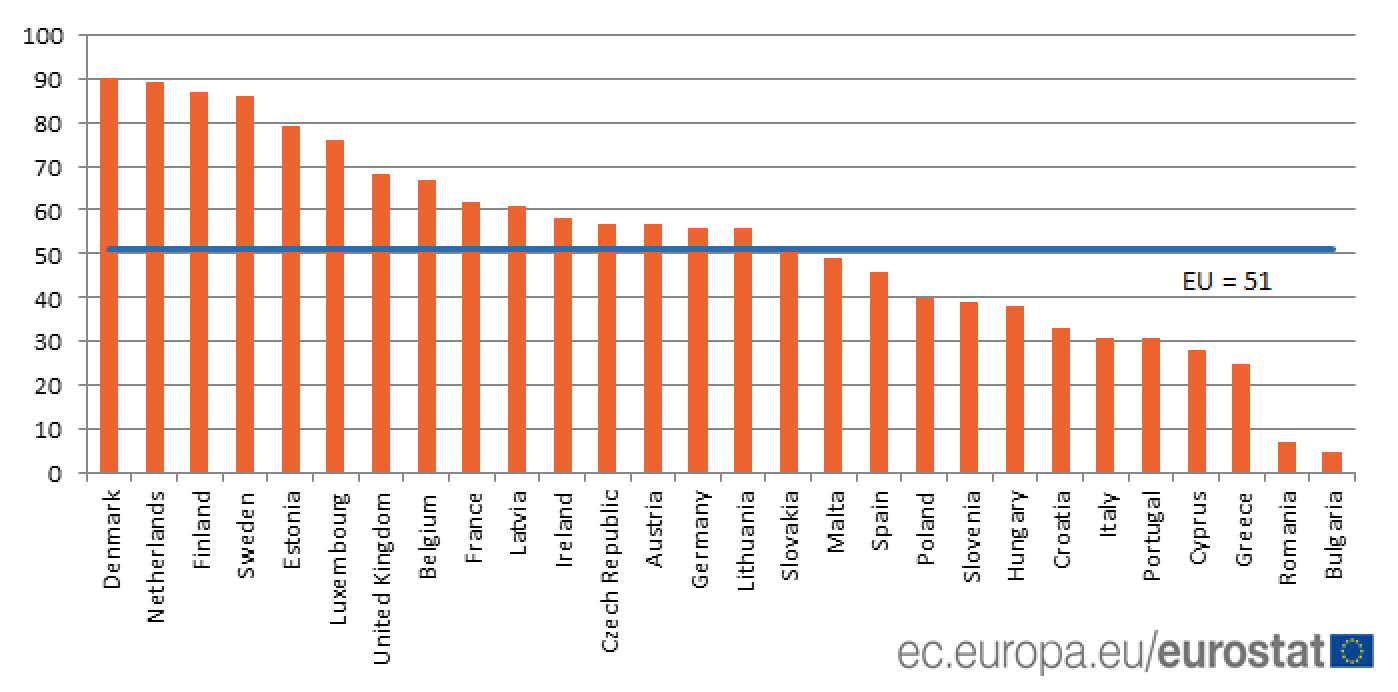
\includegraphics[width=0.8\textwidth,height=\textheight,keepaspectratio]{images/share_internet_banking.png}
    \caption{\% of individuals who used internet banking}
    \medskip
    \footnotesize\textit{Source:} "Individuals using the internet for internet banking", Eurostat, 2021.
\end{figure}

By 2017, 51\% of bank customers in European Union used internet and mobile banking at least once.
And based on the latest trends and situations, the share of internet banking will only grow.
Consequently, consumer banks are interested in offering major services via digital channels, and to research and develop modern solutions.
However, the main interest is in creating modern, and at the same time, comfortable and usual channel for user interaction, and, especially, for two-way user communication.

Obviously, the closest form of such interaction to live communication would be a form of questions and answers.
This form of interaction became widely popular due to search engines and its influence on an internet for the last decade.

People of all generations are used to asking questions on digital platforms.
Search engines have been actively developing and implementing technologies related to operating with natural languages for the last ten years.
Same engines have been studying internet users to write proper search queries to obtain expected results for decades.

\begin{figure}
    \centering
    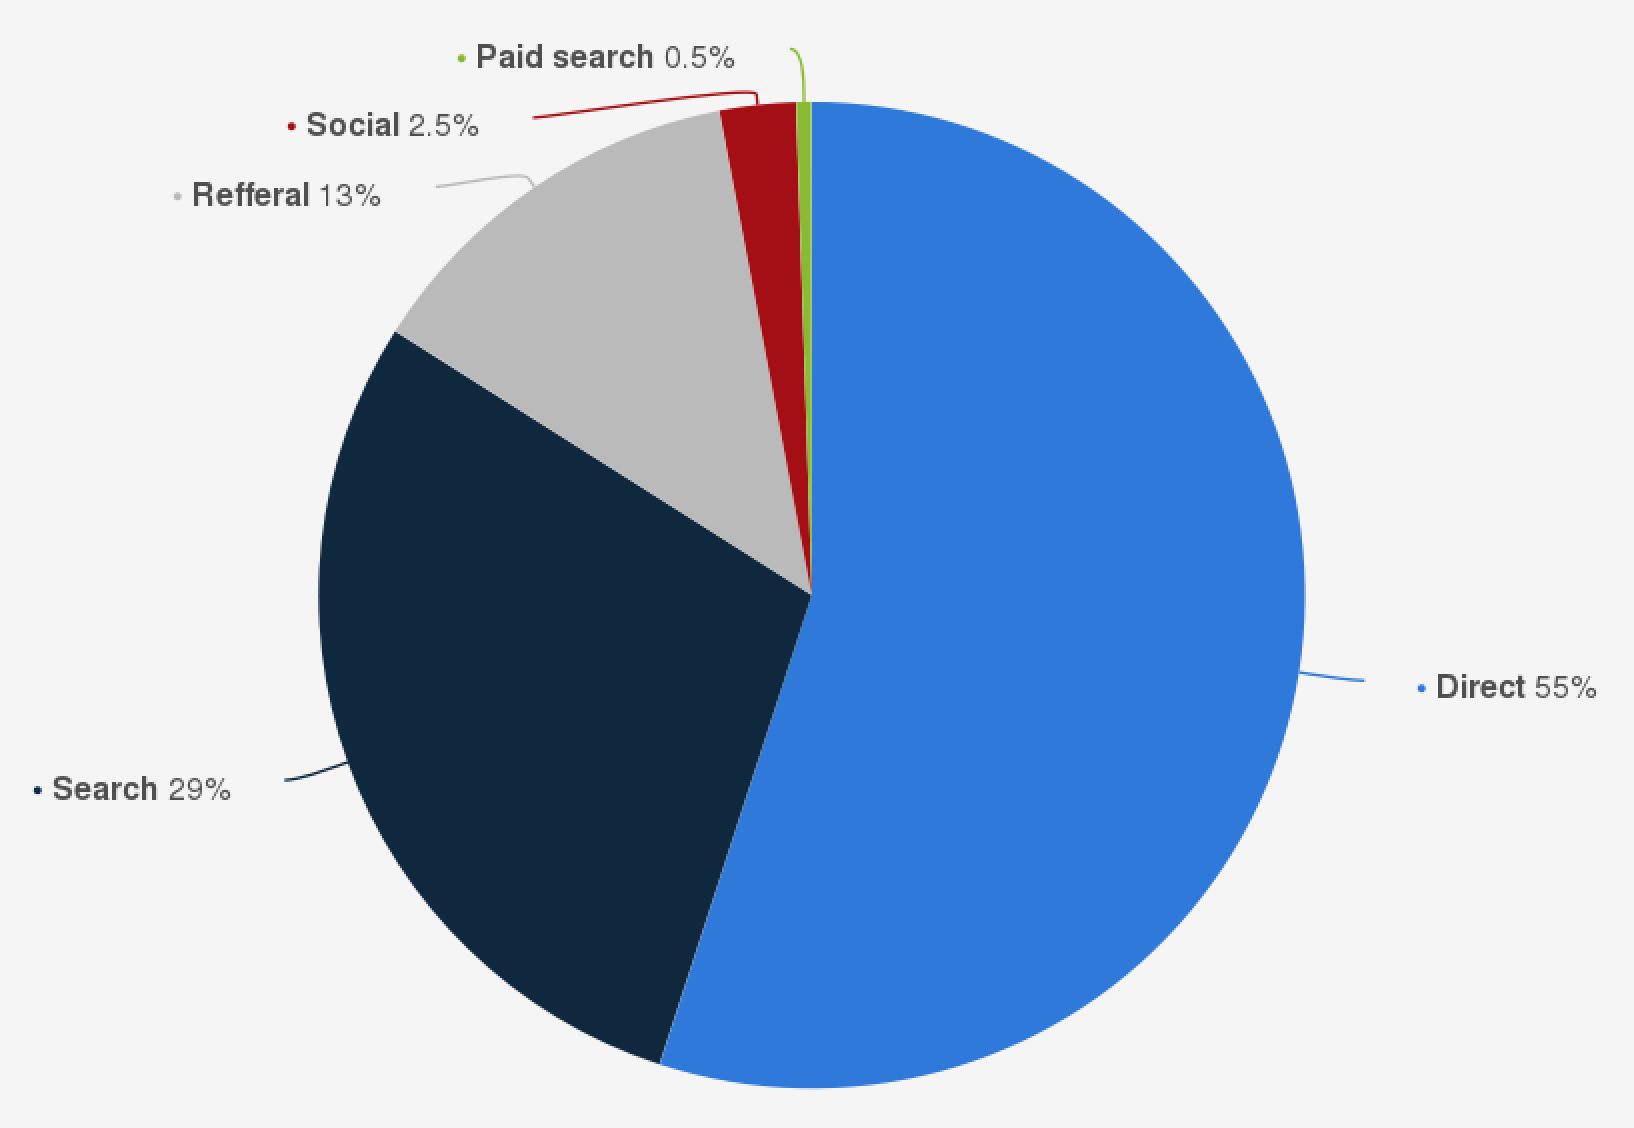
\includegraphics[width=0.8\textwidth,height=\textheight,keepaspectratio]{images/statista_search_engines.png}
    \caption{Distribution of worldwide search traffic}
    \medskip
    \footnotesize\textit{Source:} Jessica Clement "Global website traffic distribution", Statista, 2019.
\end{figure}

Nowadays, search engines have nearly 30\% of entire internet traffic.
Without ten most popular non-search engine websites this share would be around 90\%.
The influence of search engines on conversation technologies is impossible to overstate.
What is even more important, for the last ten years those technologies have been in active development and deployment, resulting in existance of a stable branch of technology with a lot of modern solutions.

Natural Language Processing is a cognitive branch of science, that investigates the application of computational techniques to the analysis and synthesis of natural language and speech.
Natural Language Processing, known as NLP, consists of Natural Language Understanding, NLU, which analysis text and finds logical points and meaning, and Natural Language Generation, NLG, which structures, plans and generates human-readable text.
Generally, NLP, both Understanding and Generation, including Voice Synthesis, became a pretty common part of technology for a user, especially due to Voice Assistants.
What is even more important, for the last ten years the cost of implementation of mentioned technologies significantly decreased.
On the contrary, amounts of investements into AI and NLP drastically increase every year.
In 2020 global NLP market value was \$1.8 billion, and is expected to grow up to \$14.4 billion by 2026.
\cite{pwc_ai_nlp}

\begin{figure}
    \centering
    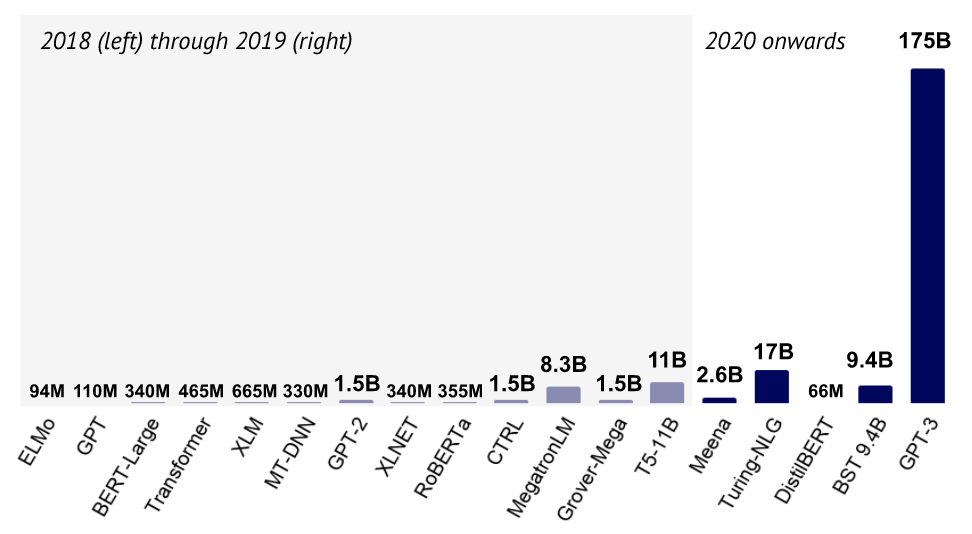
\includegraphics[width=0.8\textwidth,keepaspectratio]{images/nlp_models_parameters.png}
    \caption{Number of parameters in NLP AI algorithms}
    \medskip
    \footnotesize\textit{Source:} Nathan Benaich, Ian Hogarth "State of AI Report", stateofai.com, 2020, s. 15.
\end{figure}

It is important to highlight the exponential grow and compliction of those models. 
NLP models can have multiple billions of parameters and coefficients, that those use for text analysis and generation, with a current record of 175 billion parameters by famous GPT-3.

Main purpose of NLP with AI in this case is to replace usual contact centers and to improve customer experience.
The reason of replacement is a comparingly low conversion for existing solutions.
Contact centers are infamous for response times and low quality of solutions.
This is extremelly important, as consumers have low conversion rates if brands don't answer phone in under a minute.
Based on researches, 78\% of responsers may switch brand preferences due to poor response times, while 73\% will recommend highly responsive brands.
Additionally, 59\% of responders have extremelly high conversion rate for highly responsive brands.
\cite{lfbyphone_consumer_analytics}

At the same time, achieving positive feedback in under a minute is a main target of automated conversational banking.
Chat-bots are known for giving high conversion rates and large returns on considerable small inverstments.
\cite{accenture_ai_banking}

In consequence, banks can strive to major influence of dialog interfaces on client, through which clients can transfer funds, send it to other clients, issue card, convert currency, execute payments and various other basic tasks.

It is common to mix up Conversational banking with Mobile and Internet Banking.
However, the main difference is in user experience.
Mobile and Internet banking are hierarchical trees, both of those have a concrete form.
It is always an application, in which user can click buttons, check charts and read text in order to manipulate and make actions.
Conversational banking is much more abstract.
That is a dialog, client should not in this case know the structure of interaction.
In order to achieve something client has to have an intent and, what is even more important, to invoke an action by intention.
He doesn't need to know how to achieve something, he can just ask.
However, in this case client can rely only on his knowledge, as there would be no buttons or menus to check.

Front-office for Conversational banking may have different forms.
This can be a contact center, retail business unit for dialog-based conversation.
Couple of years ago, bank client on any problem had to call to a contact center and to talk to customer service line manager. 
\cite{trillion_opportunity}
Nowadays, there are other options.
Much more interesting option is a messenger, as a front-office for textual interactions.
In this case, this can be both a chat-bot in a popular messenger app or a social network, same chat-bot in a mobile or internet banking app, or even a voice assistant.

Currently, it is a popular solution to use chat-bots which can answer to the most simple question, but mostly transfer a conversation to the contact center.
Though, this is a not a most effective model, as client firstly has to spend his time to describe his problem to a chat-bot, and then he has to repeat to a human specialist.
\cite{accenture_conversational_banking}

\begin{table}
    \centering
    \caption{Consumer preferences for addressing issues}
    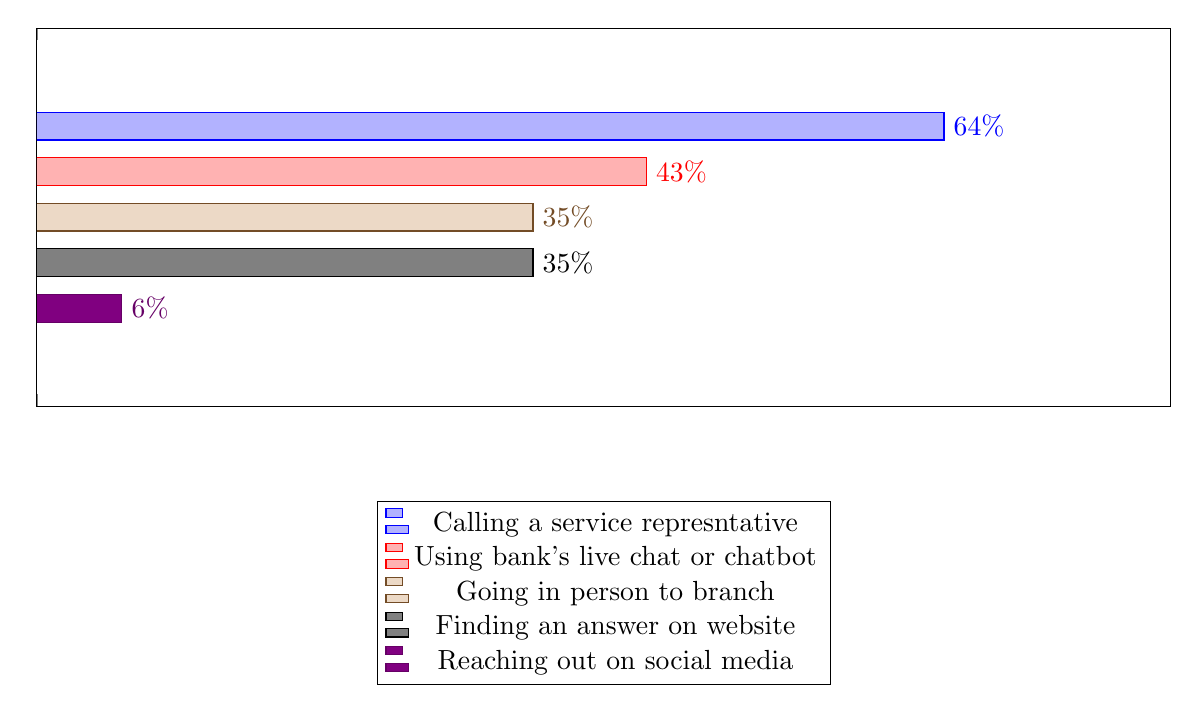
\begin{tikzpicture}
        \begin{axis} [
            xbar,
            xmin=0, xmax=80,
            x=0.18cm, y=1cm,
            xticklabels={,,},
            yticklabels={,,},
            xtick = {0}, ytick = \empty,
            nodes near coords,
            nodes near coords style={ anchor=west },
            point meta=explicit symbolic,
            legend style={at={(0.5,-0.25)},anchor=north}
        ]

        \addplot coordinates {(64,4)[64\%]};
        \addplot coordinates {(43,3)[43\%]};
        \addplot coordinates {(35,2)[35\%]};
        \addplot coordinates {(35,1)[35\%]};
        \addplot coordinates {(6,0)[6\%]};

        \legend{
            Calling a service represntative, 
            Using bank's live chat or chatbot,
            Going in person to branch,
            Finding an answer on website,
            Reaching out on social media
        }
        \end{axis}
    \end{tikzpicture}
    \medskip
    \source{Own study, based on Bill Streeter "Banking By Bot: Are Chatbots Better Than Real People?", The Financial Brand, 2018}
\end{table}
    
However, for customer it is still more comfortable to address problems via common channels of interactions, such as via phone calls or via in-person conversation in a branch.
\cite{humley_banking_report}

This is due too negative experience with current automated conversational solutions.
It is too early to talk about conversational banking in a poor form, as chat-bots are on such level of development, that those cannot be used purely, as they don't understand all the requests yet.
This results in a negative influence towards client satisfaction.

On the other side, it is important to discuss approaches to build this system.
During client conversation it is important to transfer from screen interface of mobile or internet-bank to creation of universal and operational assistant, which would be ready to interact and to help a client at any time.
This form of client interaction is based on an understanding of a global trend, as more and more people are used to talk with sellers via messengers.
Even though automated solutions are not common, those, nearly 44\% of customers would prefer to speak to chatbot, if they are sure, that a chat-bot knows an answer.
\cite{humley_banking_report}
Therefore, implementing any automatized conversational interface for a bank is impossible without influencing expectations.
This transforms entire service consumption process, as it is more comfortable to contact via suitable and familiar solutions and messengers.

Conversational banking has some significant advantages in comparison to existing systems.
Firstly, improvement of client experience. 
We can make it more comfortable, fast and qualified.
Secondly, conversational banking decreases client waiting time. 
If chat-bot is not sure about the question or the answer, dialog can be transferred to a human operator.
In case if system achieves certain level of assurance — it will reply automatically.
Researches of client experience had shown that verbal interaction is psychologically more comfortable and brings less cognitive load than visual interface.
\cite{accenture_conversational_banking}

From a practical perspective, conversational banking exists in two pure forms.
First form is a chat-bot, an automatic solution for textual communication with a client in a form of a dialog window.
The input in this case is a text provided by a user, and the output is a text returned by an analytical system, which consumes request and generates response.
Second form is a voice assistant. Internal work is analogical to a chat-bot, but it differs in a form of interaction.
Voice assistant receives spoken user messages and answers with synthesized voice responses.
Both of those forms are well known to users.
However, in most cases those are usually used as a support part and do not have sufficient level of autonomy.
Application of AI to those well known forms of interaction is the main purpose of Conversational Banking.

Consumers are used to chat and for them, it is easier than to click out their problem in an interface of website or mobile app.
The process of automation in banks is gradually growing and this, from the one side, should lead to a reduction of a number of contact center specialists.
On the other side, increasing number of customers consequently increases chat loads.
Nevertheless, increasing load shows higher client involvement.

Nonetheless, current state of AI application in Front-office has certain problems.
As it was mentioned before in \ref{subsec:ai_front_office}, conversational banking is not considered as available by middle-sized and small banks.
Mostly it is used either by the largest commercial banks, which have large amounts of resources available for investments, or by start-ups and new digital financial services, which are targeting market by innovations.

As a result, banks face a choice — use existing solutions or to create their own product, which is not available to small-sized and medium banks.
However, it is not entirely correct, as medium-sized and small banks can and have to use third-party solutions for implementation.
On the other hand, integration of external technologies uses very large volume of bank resources, as well as cost of product usage.
As a result, final cost may be higher than cost of internal development.

Another major problem is obvious and connected to existing employees in customer experience offices.
As cost decrease on customer support being a valid reason for banks, this doesn't mean that banks will decrease amount of support agents.
In contrast, those may be moved to other branches or to other banking products.
Additionally, support agents may require training for changing their profile.
The point of this action is not to decrease a number of employees, but to create a higher percentage of professionals among existing specialists.

\subsection{Hybrid approach}

Nevertheless, the largest banks already have solutions for dialog interfaces in messengers.
In those case, they are developing solutions for artificially augmented intellegence in client support.
It is a common misconception, that those chat-bots are for customers only.
Indeed, those are much more useful for bank employees as a single source of knowledge and can significantly improve client experience.
It is too early to talk about conversational banking in a poor form.

On other side, it is important to discuss approaches to build this system.
During client conversation it is important to transfer from screen interface of mobile or internet-bank to creation of universal and operational assistant, which would be ready to interact and to help a client at any time.
This form of client interaction is based on an understanding of a global trend, as more and more people are used to talk with sellers via messengers. 
This transforms entire service consumption process, as it is more comfortable to contact via suitable and familiar solutions and messengers.
Conversational banking has some significant advantages in comparison to existing systems.

Firstly, improvement of client experience. 
We can make it more comfortable, fast and qualified.
Secondly, conversational banking decreases client waiting time. If chat-bot is not sure about the question or the answer, dialog can be transferred to a human operator.
In case if system achieves certain level of assurance — it will reply automatically.
Researches of client experience had shown that verbal interaction is psychologically more comfortable and brings less cognitive load than visual interface.
Even the best market players warn — system should provide connection with a human, as there is no technology, that would allow delegating functions to computers entirely.
\cite{ways_ai_transforming_bi}

As well, chat-bot can answer by itself directly.
Unfortunately, currently it concerns only the most simple actions — customer welcoming, customer invitation, various forms of apologize, or informing the location of the nearest ATM.
If there is a large stream of clients, we can lower the system confidence threshold, in order to transfer clients to chat-bot, which could decrease waiting time and, as a result, increase client's service satisfaction.
Moreover, it is possible to involve one robot into dialogue with another robot.
For example, general support chat-bot can involve investment chat-bot.
\cite{accenture_chatbots}

\begin{table}
    \centering
    \caption{Customer Satisfaction Rate by form of Live Chat}
    \begin{tikzpicture}
        \begin{axis} [
            axis lines = middle,
            x axis line style={<->},
            smooth,
            xmin=-4, xmax=+4,
            ymin=55, ymax=92,
            xticklabels={,,},
            yticklabels={,,},
            xtick = \empty, ytick = \empty,
            ylabel = {Customer satisfaction rate},
            y label style={at={(axis description cs:0.5,1)},anchor=south},
            xlabel = {Conversion with\\Artificial Intelligence},
            x label style = {align = center, at={(axis description cs:1,0)},anchor=west},
            nodes near coords,
            nodes near coords style={ anchor=south west },
            point meta=explicit symbolic,
        ]

        \addplot+[mark=none] coordinates {
            (-4, 68)[68\%]
            (-1, 72)
            (0.1, 88)[88\%]
            (4, 60)[60\%]
        };

        \draw [dashed] (-4,68) -| (+4,68);
        \draw [dashed] (-4,88) -| (+4,88);
        \draw [dashed] (-4,60) -| (+4,60);

        \end{axis}
        
        \begin{axis} [
            axis y line = none,
            axis x line = bottom,
            xmin=-4, xmax=+4,
            ymin=55, ymax=92,
            xticklabels={,,}, yticklabels={,,},
            xtick = \empty, ytick = \empty,
            xlabel = {Conversion with\\alive agent},
            x label style = {align = center, at={(axis description cs:0,0)},anchor=east},
        ]
        \end{axis}
    \end{tikzpicture}
    \medskip
    \source{Own study, based on "Chatbots are here to stay", Accenture, 2018}
\end{table}

Conversational, dialog, bank is a hybrid between classic contact center and automated chat-bot service.
However, it is possible to use hybrid approach, in which robot recommends answer to an operator based on existing knowledge base.
Of course, the best possible answers are on top of the list, so it would be more comfortable for operator to find.
The best possible answer, in this case, would be an answer of the most competent expert, which would allow for an intern to answer on professional level.
Every client question and every operator answer are stored in database and is a template for future answers.
Operators are teachers and database is a student, and this is the way AI learns.
Of course, it requires specialists to develop such a system.

Similar augmentative system can be virtual broker, which give hints based on AI and can pick up an individual way to each client.
Nonetheless, there can be a personal-manager service, which communicates in chat and can execute large number of operations.
This may decrease loads, manual work, to transfer payments form from a manager to an AI.
Human-in-the-loop or HITL — a system, in which there should be a person for a proper functioning.
Specialist can choose various relevant actions.
Manager answers with text messages, as well as with special widgets with portfolio description or with operation confirmation. 


Artificial Intelligence has already become a leading driver for technology innovations in banking sector.
It has already been developed enough and definitely reliable in everything regarding risks, confidentiality, human factor and marketing strategies.

Nevertheless, AI has already changed financial business and will change it even more in near future.
The vast majority of actions, that are being done both in back-office, middle-office and front-office by employees can be automated and algorithmized.

\mttable
{FinTech AI Use-cases}
{Own study, based on: Lex Sokolin, Matt Low, "\#Machine Intelligence \& Augmented Finance", \allowbreak Autonomous Research, p. 29.}
{
    \begin{tabular}{| c | c | c | c |}
        \hline 
        \textbf{Divisions} &
            Front office & 
            Middle office & 
            Back office \\ \hline 
       
        \textbf{More mature} & 
            Conversational banking & 
            Anti-fraud, KYC, AML & 
            Credit underwriting \\ \hline 
       
        \textbf{Less mature} & 
            Biometrics & 
            Legal and Compliance &
            Smart contracts \\ \hline 
        \textbf{Savings} &
            \$199 billion &
            \$217 billion &
            \$32 billion \\
        \hline 
    \end{tabular}
}

The main interest for banks is in application of AI in front-office and middle-office, as it will lead to significant cost reduction, up to \$400 billion in 2025.
Banks use AI in front-office for identification and authentication of clients, in order to imitate alive workers with chatbots and voice assistants, to deepen relationships with customer, increase engagement, and to offer personalized ideas and recommendations.
Additionally, AI is being used in middle-office.
It allows detecting and preventing frauds with payments, upgrading processes connected to anti-money laundering processes and detection for know your customer control systems.
Those sources of income, which have already been transformed by AI, show the valid way to use this possibility.
Nevertheless, those strategies show that banks have to create holistic strategy, which would connect and cover multiple scopes of banking, sources of useful data, third-parties and employees.
\cite{autonomous_next}

However, with all the advantages of modern software, forecasts of full robotization probably won't be realized, as in near future it is unlikely for a program to replace a person.
\cite{deluxe_mid_size_banks_risk}

In order to integrate the foregoing into existing banking service it is necessary for banking platform to support it.
Obviously, those platforms, which current banking stands on were developed around 15-30 years ago, or even more, and this makes integration of modern algorithms almost impossible. 
This is why modern banks are now puzzled if it is possible to re-engineer their software in order to have an effective possibility to embed Artificial Intelligence and Machine Learning in its banking platform.

Nevertheless, it is extremely important to remember, that automating workplaces doesn't always lead to dismissal of workers.
It is important to create retraining programs, that would allow existing employees to obtain new skills in fields,
that are out of risk of automation, in order to decrease automation's influence on labor market.

Increasing number of internet users, availability of smartphones and other handheld devices, and rapid development of mobile internet forms new users' habits and behaviors.
Social network users and mobile app users are more and more focused on getting instant results and target specific actions with the lowest amount of clicks possible.

However, the need of receiving high-quality financial services and personal consultations hasn't disappeared: people are still calling to call-centers.
Even though remote banking service systems are rapidly developing, number of phone calls recently significantly increased. 

Nevertheless, there are good news for banks that have yet to embark on their AI journey. 
Making progress in AI does not require an unbearable effort.
It typically begins with identifying your organizational goals, readying your data and finding the right partners.
Nonetheless, even medium-sized and small banks have to investigate this topic by now, as in future, gap between AI users and nonuser will only widen.





